\documentclass[times, utf8, zavrsni]{fer}
\usepackage{booktabs}
\usepackage{subfig}
\begin{document}

% TODO: Navedite broj rada.
\thesisnumber{3948}

% TODO: Navedite naslov rada.
\title{Raspoznavanje objekata konvolucijskim neuronskim mrežama}

% TODO: Navedite vaše ime i prezime.
\author{Dario Smolčić}

\maketitle

% Ispis stranice s napomenom o umetanju izvornika rada. Uklonite naredbu \izvornik ako želite izbaciti tu stranicu.
\izvornik

% Dodavanje zahvale ili prazne stranice. Ako ne želite dodati zahvalu, naredbu ostavite radi prazne stranice.
\zahvala{}

\tableofcontents

\chapter{Uvod}
Računalni vid je područje koje uključuje metode za dohvaćanje, obrađivanje i shvaćanje slika i općenito podataka velikih dimenzija te je zanimljivo područje računalne znanosti zbog mogućnosti široke primjene u današnjem svijetu. Jedna od podgrana ovog područja je raspoznavanje objekata.

Ljudi su sposobni prepoznati mnoštvo različitih objekata sa jako malo truda no za računala je to složen proces koji ima brojna ograničenja koja ljudi nemaju. Uzmimo u obzir da se slika u računalu reprezentira kao višedimenzionalni niz jačina svjetlosti. Promjene u prikazu objekta poput različite orijentacije, skaliranja, i osvijetljenja objekta su u digitalnim slikama prestavljene sa različitim podatcima. Objekt također može biti i zaklonjen. Dobar model raspoznavanja mora biti otporan na ove varijacije te je zato problem raspoznavanja objekata još uvijek neriješen i u zadnjih nekoliko desetljeća su razvijene brojne metode kojima se pokušava riješiti ovaj problem.
Za razliku od pisanja klasičnih algoritama poput sortiranja brojeva za problem klasifikacije objekata nije očito kako bi se mogao napisati takav algoritam gdje su sve varijacije ulaza posebno obrađene u kodu. Zato se za klasifikaciju objekata koristi pristup usmjeren na podatke (engl. \textit{data-driven approach}). Programu se da veliki broj ulaza sa velikom količinom primjera za svaku klasu te se razvije algoritam učenja koji učitava date primjere te uči o vizualnom prikazu svake klase. Takve programe nazivamo klasifikatorima.

U zadnjih nekoliko desetljeća su razvijeni različiti klasifikatori za što točnije prepoznavanje objekata. Među tim klasifikatorima su i umjetne neuronske mreže. Ispostavilo se da se sa dubokim neuronskim mrežama trenutno dobivaju najbolji rezultati za problem klasifikacije. Najkorišteniji oblik dubokih neuronskih mreža u račnunalnom vidu su konvolucijske neuronske mreže.

Cilj ovog rada je razviti implementaciju konvolucijske neuronske mreže za primjenu na osobnim računalima, optimirati hiperparametre mreže te vrednovati učinak naučene mreže. Razvijena mreža će se testirati na skupu MNIST rukom pisanih znamenki.
\chapter{Neuronske mreže}
Područje umjetnih neuronskih mreža (engl. \textit{Artificial Neural Networks - ANN}) je prvotno bilo inspirirano sa modeliranjem biološkog živčanog sustava, a tek kasnije se počelo koristiti u sklopu strojnog učenja. 
\section{Neuron}
Radi razumijevanja neuronske mreže potrebno je prvo razumijeti funkcioniranje jednog neurona. Ljudski živčani sustav se sastoji od otprilike 86 bilijona neurona koji su povezani sa $10^{14}$ do $10^{15}$ sinapsi. Svaki neuron dobiva svoje ulazne signale kroz dendrite i šalje izlazni signal kroz akson. Akson je sa sinapsama spojen sa dendritima drugih neurona. Na slici ~\ref{fig:bio-neuron} možemo vidjeti izgled biloškog neurona.
\begin{figure}
    \centering
    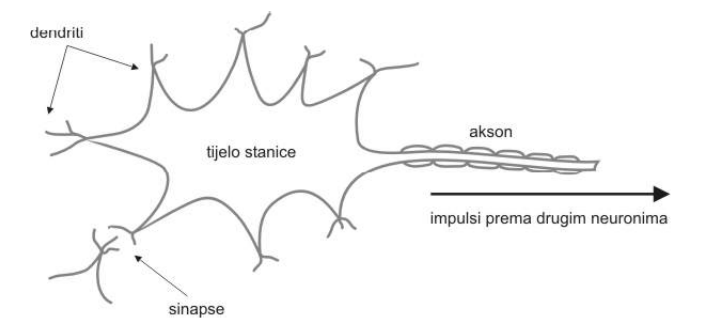
\includegraphics[width=12cm]{img/bio-neuron.png}
    \caption{Biološki neuron}
    \label{fig:bio-neuron}
\end{figure}

U modelu umjetnog neurona signali koji putuju aksonom (npr. \textbf{$x_{0}$}) se množe sa sinaptičkim snagama dendrita(težinama) drugih neurona (npr. \textbf{$w_{0}$}). Ideja je da se sinaptičke snage mogu mijenjati sa učenjem te određuju utjecaj jednog neurona na drugi. Svaki neuron ima aktivacijsku funkciju koja uzima sumu umnoška ulaza neurona sa pripadnim težinama i praga ($\theta$) te ih preslikava na izlaz neurona koji modelira signal na aksonu($y$). Na slici ~\ref{fig:umj-neuron} možemo vidjeti model umjetnog neurona. 
\begin{figure}
    \centering
    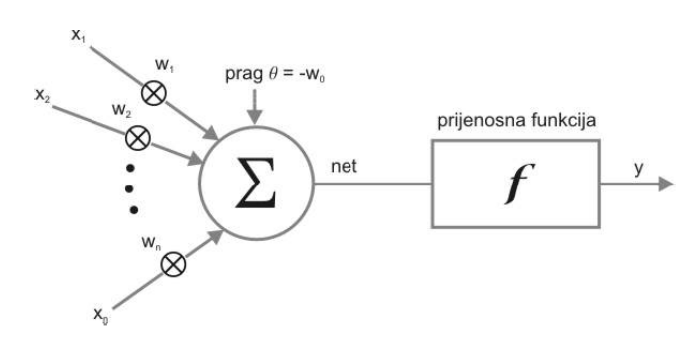
\includegraphics[width=12cm]{img/umj-neuron.png}
    \caption{Umjetni neuron}
    \label{fig:umj-neuron}
\end{figure}

Označimo ulaze sa $x_{1},x_{2},...,x_{n}$ te njihove pripadne težine sa $w_{1},w_{2},...,w_{n}$, i prag sa $\theta$. Onda možemo izlaz neurona zapisati kao:
$$ y = f(\displaystyle\sum_{i=0}^{n}(x_i*w_i) + \theta) $$
Radi pojednostavljenja se često uzima oznaka $w_0$ umjesto $\theta$ te se dodaje jedan ulaz $x_0$ koji je stalno jednak 1. Sa ovom modifikacijom izlaz se može izraziti kao:
$$ y = f(\displaystyle\sum_{i=0}^{n}(x_i*w_i)) $$
\subsection{Aktivacijske funkcije}
Postoje veliki izbor aktivacijskih funkcija no u praksi se koriste samo neke koje su se pokazale korisnima. Spomenuti ćemo četiri različite aktivacijske funkcije (slika ~\ref{fig:aktivacijske-funkcije}) te njihove karakteristike.

Najobičnija aktivacijska funkcija je linearna aktivacijska funkcija koja je preslikava svoj ulaz na izlaz. Ovakav tip aktivacijske funkcije ne koristimo u dubokim neuronskim mrežama zato što onemogućava učenje mreže. Step funkcije u neuronima funkcioniraju kao prekidači. Izlaz funkcije može poprimiti samo dvije različite vrijednosti ovisno o tome da li je ulaz manji ili veći od nekog praga. Ovakva funkcija je korisna za binarnu klasifikaciju.
$$ y = \begin{pmatrix}
  a_{1,1} & a_{1,2} & \cdots & a_{1,n} \\
  a_{2,1} & a_{2,2} & \cdots & a_{2,n} \\
  \vdots  & \vdots  & \ddots & \vdots  \\
  a_{m,1} & a_{m,2} & \cdots & a_{m,n}
 \end{pmatrix}
$$

\subsection{Duboke neuronske mreže}
pensi
\subsection{Algoritam backpropagation}


\chapter{Konvolucijske neuronske mreže}

\subsection{Struktura mreže}
\subsubsection{Konvolucijski slojevi}
\subsubsection{Slojevi sažimanja}
\subsection{Hiperparametri mreže}




\chapter{Zaključak}
Zaključak.

\bibliography{literatura}
\bibliographystyle{fer}

\begin{sazetak}
Sažetak na hrvatskom jeziku.

\kljucnerijeci{Ključne riječi, odvojene zarezima.}
\end{sazetak}

% TODO: Navedite naslov na engleskom jeziku.
\engtitle{Title}
\begin{abstract}
Abstract.

\keywords{Keywords.}
\end{abstract}

\end{document}
